% FROZEN --- the five Appendix D circuit-figure captions as they stood before
% the cards replaced them.  Not \input by anything: this file exists so that
% code/_build_povm_cards.py's assertion 23 ("nothing printed today vanishes")
% still has the captions to check the cards' parameter blocks against, now
% that bsc-thesis.tex no longer carries them.  Never edited.
\begin{figure}[H]
\centering
$$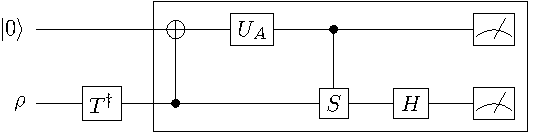
\includegraphics{figures/circuit_dec_tet.pdf}$$
\caption{Circuit for the tetrahedral POVM~\cite[Fig.~7]{decker2004quantumcircuitssinglequbit}. The CNOT implements the permutation $Q^\dagger$ with $\ket{00}\mapsto\ket{00}$, $\ket{11}\mapsto\ket{01}$. The inter-orbit unitary on the ancilla is $U_A = \sqrt{2}\bigl(\begin{smallmatrix}\alpha & \beta \\ \beta & -\alpha\end{smallmatrix}\bigr)$ with $\alpha = \sqrt{(3+\sqrt{3})/12}$ and $\beta = \sqrt{(3-\sqrt{3})/12}$. The ancilla-controlled $S = \mathrm{diag}(1,i)$ realizes the diagonal phase correction $\mathrm{diag}(1,1,1,i)$, and $H = \mathsf{F}_2$ is the Hadamard. In symbols, $\tilde{M}^\dagger = (I_2 \otimes \mathsf{F}_2)\,\mathrm{diag}(1,1,1,i)\,(U_A \otimes I_2)\,Q^\dagger$. All four computational outcomes carry non-zero probability. Uniquely among the five solids the reorientation $T^\dagger$ also carries outcome $k$ to vertex $k$ of Table~\ref{tab:povm-atlas}, so no relabelling follows. Figure~\ref{fig:tet_povm_circuit} is this circuit with the optional $U_g$ restored.}
\label{fig:dec_tet_circuit}
\end{figure}

\begin{figure}[H]
\centering
$$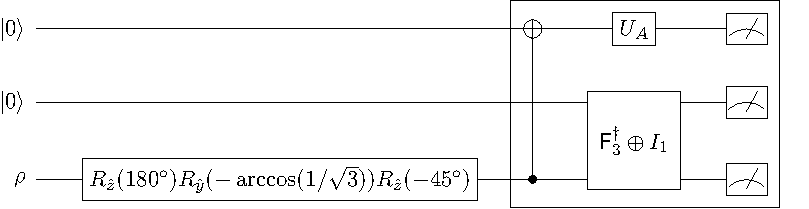
\includegraphics{figures/circuit_dec_oct.pdf}$$
\caption{Circuit for the octahedral POVM~\cite[Fig.~11]{decker2004quantumcircuitssinglequbit}. The CNOT realizes the permutation $Q_8^\dagger$ with $\ket{000}\mapsto\ket{000}$ and $\ket{101}\mapsto\ket{001}$. The inter-orbit unitary is $U_A = \sqrt{3}\bigl(\begin{smallmatrix}\alpha & \beta \\ \beta & -\alpha\end{smallmatrix}\bigr)$ with $\alpha = \sqrt{(3+\sqrt{3})/18}$ and $\beta = \sqrt{(3-\sqrt{3})/18}$. The $3$-point Fourier transform is embedded into the lower two-qubit register as $\mathsf{F}_3^\dagger \oplus I_1 \in \C^{4 \times 4}$. In symbols, $\tilde{M}^\dagger_8 = (U_A \otimes (\mathsf{F}_3^\dagger \oplus I_1))\,Q_8^\dagger$. Six of the eight computational outcomes carry non-zero probability. The reorientation is the one of the five about no coordinate axis, its three-fold face normal having to swing onto a vertex; outcomes are then relabelled by a fixed permutation in post-processing.}
\label{fig:dec_oct_circuit}
\end{figure}

\begin{figure}[H]
\centering
$$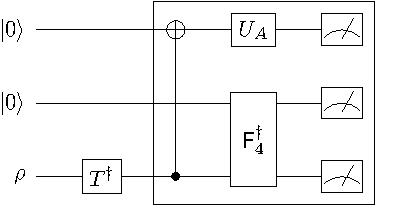
\includegraphics{figures/circuit_dec_cube.pdf}$$
\caption{Circuit for the cubic POVM~\cite[Fig.~9]{decker2004quantumcircuitssinglequbit}. The CNOT realizes the permutation $Q^\dagger$ with $\ket{000}\mapsto\ket{000}$ and $\ket{101}\mapsto\ket{001}$. The inter-orbit unitary is $U_A = 2\bigl(\begin{smallmatrix}\alpha & \beta \\ \beta & -\alpha\end{smallmatrix}\bigr)$ with $\alpha = \sqrt{(3+\sqrt{3})/24}$ and $\beta = \sqrt{(3-\sqrt{3})/24}$. The $4$-point Fourier transform $\mathsf{F}_4^\dagger$ acts on the lower two-qubit register. In symbols, $\tilde{M}^\dagger = (U_A \otimes \mathsf{F}_4^\dagger)\,Q^\dagger$. All eight computational outcomes carry non-zero probability. The reorientation is the tetrahedron's same eighth-turn, these being the two solids whose axis orders already agreed; outcomes are then relabelled by a fixed permutation in post-processing.}
\label{fig:dec_cube_circuit}
\end{figure}

\begin{figure}[H]
\centering
$$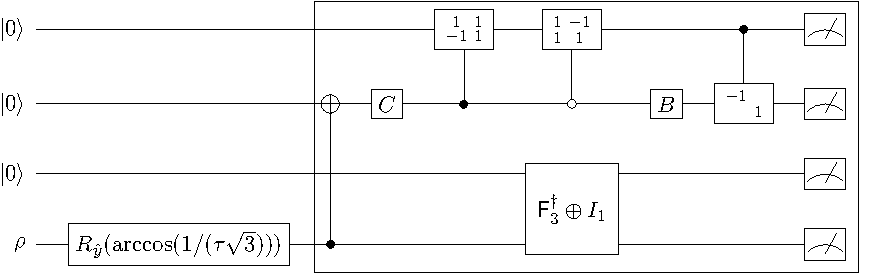
\includegraphics{figures/circuit_dec_icos.pdf}$$
\caption{Circuit for the icosahedral POVM~\cite[Fig.~15]{decker2004quantumcircuitssinglequbit}. The CNOT realizes the permutation $Q_{16}^\dagger$ with $\ket{0000}\mapsto\ket{0000}$ and $\ket{0101}\mapsto\ket{0001}$. The two-qubit unitary $A^\dagger$ acting on the top two wires factors as $A^\dagger = (I_2 \oplus (-\sigmaz))\,(I_2 \otimes B)\,R\,(I_2 \otimes C)$, where $C = \bigl(\begin{smallmatrix}v_- & v_+ \\ v_+ & -v_-\end{smallmatrix}\bigr)$, $B = \bigl(\begin{smallmatrix}u_- & -u_+ \\ u_+ & u_-\end{smallmatrix}\bigr)$, and $R$ is the product of the two controlled rotations shown---each $\pm 1$ entry in those rotation boxes denotes $\pm\sqrt{1/2}$. The diagonal-matrix box $\mathrm{diag}(-1, 1) = -\sigmaz$, controlled by the top wire, realizes $I_2 \oplus (-\sigmaz)$ on the upper two-qubit register. The constants are $u_\pm = \tfrac{1}{10}\sqrt{50 \pm 5\sqrt{10(5 + \sqrt{5})}}$ and $v_\pm = \mp\tfrac{1}{2}\sqrt{2 \pm \sqrt{5/3} \mp \sqrt{1/3}}$, and $A = \sqrt{3}\bigl(\begin{smallmatrix}\alpha & \beta & \gamma & \delta \\ \beta & -\alpha & \delta & -\gamma \\ \gamma & -\delta & -\alpha & \beta \\ \delta & \gamma & -\beta & -\alpha\end{smallmatrix}\bigr)$ with $\alpha, \beta, \gamma, \delta$ rescaled by $\sqrt{1/6}$ from the values introduced in the chapter intro. The Fourier block $\mathsf{F}_3^\dagger \oplus I_1$ acts on the lower two wires. In symbols, $\tilde{M}_{16}^\dagger = (A^\dagger \otimes (\mathsf{F}_3^\dagger \oplus I_1))\,Q_{16}^\dagger$. Twelve of the sixteen computational outcomes carry non-zero probability. Outcomes are then relabelled by a fixed permutation in post-processing.}
\label{fig:dec_icos_circuit}
\end{figure}

\begin{figure}[H]
\centering
$$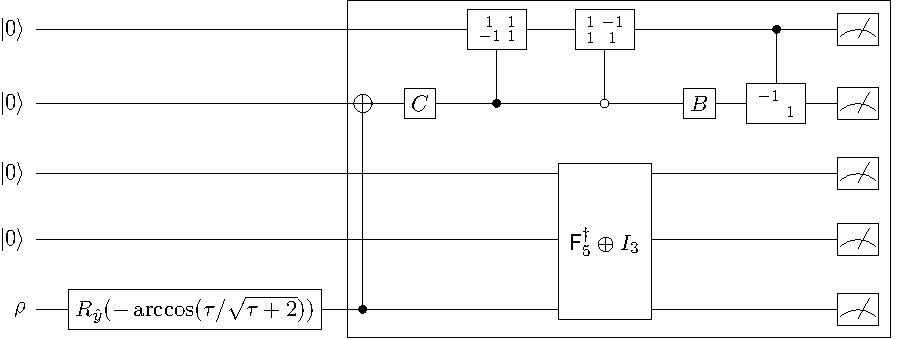
\includegraphics{figures/circuit_dec_dodec.pdf}$$
\caption{Circuit for the dodecahedral POVM~\cite[Fig.~13]{decker2004quantumcircuitssinglequbit}. The CNOT realizes the permutation $Q_{32}^\dagger$ with $\ket{00000}\mapsto\ket{00000}$ and $\ket{01001}\mapsto\ket{00001}$. The two-qubit unitary $A^\dagger$ on the top two wires has the same factorization as in Figure~\ref{fig:dec_icos_circuit}; the rotation entries $\pm 1$ again denote $\pm\sqrt{1/2}$. The constants here are $u_\pm = \sqrt{\tfrac{1}{2} \pm \sqrt{\tfrac{3+\sqrt{5}}{24}}}$ and $v_\pm = \mp\sqrt{\tfrac{1}{2} \pm \sqrt{\tfrac{\sqrt{5}-1}{8\sqrt{5}}}}$, and $A = \sqrt{5}\bigl(\begin{smallmatrix}\alpha & \beta & \gamma & \delta \\ \beta & -\alpha & \delta & -\gamma \\ \gamma & -\delta & -\alpha & \beta \\ \delta & \gamma & -\beta & -\alpha\end{smallmatrix}\bigr)$ with $\alpha, \beta, \gamma, \delta$ rescaled by $\sqrt{1/10}$ (recall $\gamma$ and $\delta$ are exchanged relative to the icosahedron). The Fourier block $\mathsf{F}_5^\dagger \oplus I_3$ acts on the lower three wires. In symbols, $\tilde{M}_{32}^\dagger = (A^\dagger \otimes (\mathsf{F}_5^\dagger \oplus I_3))\,Q_{32}^\dagger$. Twenty of the thirty-two computational outcomes carry non-zero probability. Outcomes are then relabelled by a fixed permutation in post-processing.}
\label{fig:dec_dodec_circuit}
\end{figure}

